\chapter{A MACHINE LEARNING BASED APPROACH TO QUANTIFYING NOISE IN MEDICAL IMAGES}
\label{chap:SPIE1}

\let\thefootnote\relax\footnotetext{
Parts of this chapter previously appeared as:
A. Chowdhury, K.~S. Aggour, S.~M. Gustafson, B. Yener,
``A Machine Learning Approach to Quantifying Noise in Medical Images.''
\emph{Medical Imaging 2016: Digital Pathology},
vol. 9791, pp. 979110U, 2016.}

%%% INTRODUCTION
\section{Introduction}

This chapter is the first of the two works that focus on quantification of the contributions of components of the image classification pipeline. As shown in Fig. \ref{fig:chapter4}, we quantify the quality of the images or the image dataset. Here, we show how we can use a machine learning based score to quantify the noise in the image sample itself. 

\begin{figure}[ht!]
\centering
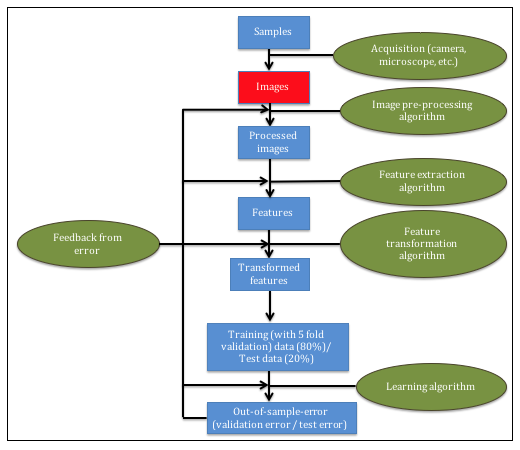
\includegraphics[width=1.0\textwidth]{img/chapter4}
\caption{Quantification of the quality of the image or image datasets. In this chapter, we quantify the quality or the contribution of the image or images in the dataset used for image classification. This layer is highlighted as red in the figure.}
\label{fig:chapter4}
\end{figure}


As advances in medical imaging technology are resulting in significant growth of biomedical image data, new techniques are needed to automate the process of identifying images of low quality. Automation is needed because it is very time consuming for a domain expert such as a medical practitioner or a biologist to manually separate good images from bad ones. While there are plenty of de-noising algorithms in the literature, their focus is on designing filters which are necessary but not sufficient for determining how useful an image is to a domain expert.
Thus a computational tool is needed to assign a score to each image based on its perceived quality. In this chapter, we introduce a machine learning-based score and call it the \textit{Quality of Image (QoI)} score. The \textit{QoI} score is defined based on the probabilities of classification using the logistic regression classifier.
We test our technique on clinical image data obtained from cancerous tissue samples. We used 723 tissue samples that are stained by three different markers (abbreviated as CK15, pck26, E\_cad) leading to a total of 2,169 images. Our automated labeling is in agreement with the domain experts with an F1-score of 0.9044 on average. The results show a distribution of the \textit{QoI} score for each of the three markers that correspond to the actual quality of the images from the marker according to the pathologist who labelled the images based on their perceived quality.  We also quantify the quality of the markers and their differences based on the \textit{QoI} scores of each sample stained using that marker. 
Furthermore, we propose a data-driven method by which images maybe recovered based on the \textit{QoI} score and forwarded for further post-processing.

%%% Data
\section{Data}

The data we use is in the form of microscopic images. The colon cohort in this analysis was collected from the Clearview Cancer Institute of Huntsville Alabama from 1993 until 2002, with 747 patient tumor samples collected as formalin-fixed paraffin-embedded specimens. The median follow-up time of patients in this cohort is 4.1 years, with a maximum of over ten years. Stage 2 patients comprise 38 \% of this cohort, stage 1 and 2 combined are 65 \% of the total patients. We have stained and processed 747 CRC subjects described above on tissue microarrays for 63 target proteins of consequence to cancer biology and ancillary image processing and analysis. A full description of materials and methods was described recently in \cite{gerdes2013highly}.
The images in this work are stained with three different markers. The markers are Ecadherin (E\_cad), pan-Keratin (pck26) and Keratin15 (CK15). The three markers stain epithelial cells in the tissue. The raw dataset consists of 747 tissue samples and each tissue sample has four images from each marker; resulting in a total of 2,988 images.  723 images from the 747 samples were selected by the pathologist for this work which result in a total of 2169 images from all the 3 stains.
The images marked with E\_cad have the least amount of noise associated with them. Images stained with pck26 is more noisy than E\_cad, while CK15 is the noisiest among the 3 markers with respect to the presence of undesirable artifacts in the image. This difference in quality maybe observed from Fig. \ref{fig:example_images} from each of the 3 protein markers. We quantify the quality of  both images and markers using the \textit{QoI} score defined in this chapter. 

\begin{figure}
    \centering
    \begin{subfigure}[b]{0.3\textwidth}
        \centering
        \includegraphics[width=\textwidth]{img/SPIE/ecad_example.eps}
        \caption{E\_cad}
        \label{fig:ecad_example}
    \end{subfigure}
    \hfill
    \begin{subfigure}[b]{0.3\textwidth}
        \centering
        \includegraphics[width=\textwidth]{img/SPIE/pck26_example.eps}
        \caption{pck26}
        \label{fig:pck26_example}
    \end{subfigure}
    \hfill
    \begin{subfigure}[b]{0.3\textwidth}
        \centering
        \includegraphics[width=\textwidth]{img/SPIE/CK15_example.eps}
        \caption{CK15}
        \label{fig:CK15_example}
    \end{subfigure}
    \caption{Examples of a single colon tumor tissue sample stained with three different markers. E\_cad is the least noisy with respect to undesirable artefacts, followed by pck26 and CK15 respectively.}
    \label{fig:example_images}
\end{figure}

\subsection{Feature extraction}

We quantify the information in the three markers (E\_cad, pck26, CK15) by texture features. Texture based features maybe used as a way to quantify the difference between images based on amount of signal or noise in an image, and be able to distinguish between images of the types shown in Fig. \ref{fig:example_images} .  These set of 13 features are based on gray-level intensity values, and texture information \cite{haralick1979statistical, haralick1973textural} in the images. 
Haralick features \cite{Haralick1973} are calculated using gray-level co-occurrence matrices (\textit{G$_{ij}$}, shown below) which are square matrices of size \textit{N$_g$} x \textit{N$_g$}, where \textit{N$_g$} is the number of gray levels in an image:
\\
\begin{equation}
%\[
G_{ij}=
  \begin{bmatrix}
    p(1,1) & p(1,2) & \cdots       & p(1,N_{g}) \\
    p(2,1) & p(2,2) &  \cdots      & p(2,N_{g}) \\
     \vdots &  \vdots &  \ddots    &  \vdots          \\
    p(N_{g},1)  & p(N_{g},2) & \cdots & p(N_{g},N_{g}) 
  \end{bmatrix}
%\]
\end{equation}
\\
Each matrix element, $ \ [i,j]\ $, is calculated by counting the number of times a pixel with value \textit{i} is adjacent to pixel with value \textit{j}.  When considering a square pixel image, there are four directions for which a gray-level co-occurrence matrix can be calculated: horizontal, vertical, left diagonal, and right diagonal.  Haralick texture statistics can be calculated based on the four gray-level co-occurrence matrices from each of these four directions. Haralick features thus describe the texture of an image. Fundamentally, texture is the arrangement of a certain feature or property, relative to the environment. In images, texture is the spatial distribution (arrangement) of gray-level variations in an image. Haralick features, computed from image gray-level co-occurrence matrices, capture texture patterns in an image. 

In addition to the features, labels are assigned to each image by domain experts based on the amount of noise in them. The label +1 is assigned if the image has some signal in it. This class is colloquially referred to as the \textit{good} class.  Images with a lot of noise in them where there is almost no signal are labelled as -1 or the \textit{bad} class.

\subsection{Data preprocessing}
The three markers (CK15, pck26, E\_cad) corresponding to each tissue sample are combined together to provide us with 723 x 3 = 2169 samples. We perform 5-fold cross validation on this data to compute the quality of image score and report the accuracy and F1-score on the validation data.
The data is highly imbalanced. The ratio of bad to good images is roughly 1 : 18. Therefore, it is important to try to redress this imbalance. We use the synthetic minority oversampling technique (SMOTE) \cite{chawla2002smote} on this data to perform oversampling.  In this data balancing technique, the minority class (\textit{bad}) is oversampled by introducing synthetic samples along the line joining any or all of the \textit{k} minority class nearest neighbors. Here \textit{k} is set as 5. The number of neighbors from the \textit{k} - nearest neighbors are randomly chosen depending on the amount of oversampling needed.

Principal components analysis (PCA) \cite{wold1987principal} is performed to reduce the number of features from 13 such that it captures 95 \% of the information. This reduces the number of dimensions to 5.
PCA is a feature transformation technique that uses orthogonal transformation to convert a set of observations of correlated variables to linearly uncorrelated ones. These orthogonal components are called principal components. PCA can be thought of as a transformation that reveals the structure of the data in a way that best explains the variance in the data. The drawback of this technique is that the features obtained after reduction are linear combinations of the original feature variables which occupy a different vector space than the original variables. 


\section{Methods and experiments}
In this section, we describe the methods that we used in our analysis of the images and also show the results that we achieved from the application of these methods on our data.

\subsection{Classification and analysis}
The features from all the 3 markers are combined to form a feature matrix of size 2169 x 5 (after dimensionality reduction using PCA). We combine the data together for two reasons. The first reason is that this provides more samples for training. The second reason is that we want to create a quantity that quantifies the score over all the markers and is not just trained on one marker. 
We used the logistic regression classification algorithm for performing classification. We choose the logistic regression algorithm because it is a simple classification algorithm that can make binary decisions. In addition, the sigmoid function used in logistic regression, squashes the the output of the linear function between 0 and 1. This value can be directly interpeted as a probability. This is exactly what we define as the \textit{QoI} score in Eq. \ref{eq:1} defined in the next section.
The F1-score for classification using the feature matrix on the binary classification problem is 0.9044 ($\pm$  0.03 standard deviation). We use the F1-score instead of accuracy as the classification metric because of the imbalance in the dataset.

\subsection{Quality of image score}
The \textit{Quality of Image (QoI)} score is defined as the probability that an image is from the \textit{good} class. It is given by Eq. \ref{eq:1}.
\begin{equation}
\begin{gathered} 
S_i \ =  \ p_{i1} 
\end{gathered}
\label{eq:1}
\end{equation}
A high value of the probability indicates that the image has high quality and must be used for further analysis. A low value of the probability denotes that the image belongs to the \textit{bad} class and it can be discarded. An intermediate value of the probability is interesting because it denotes there is some signal in the image and that it may or may not be used for analysis. We define such an image to be \textit{ugly} which is neither \textit{good} nor \textit{bad}.
 The three sample images in the following figure show examples of images from the validation dataset that can be considered as \textit{good}, \textit{bad} and \textit{ugly} according to the \textit{QoI} score. 

\begin{figure} [ht!]
    \centering
    \begin{subfigure}[b]{0.3\textwidth}
        \centering
        \includegraphics[width=\textwidth]{img/SPIE/E_cad_AFRemoved_260143_9945.eps}
        \caption{A \textit{good} image from E\_cad marker with a \textit{QoI} of 0.9945}
        \label{fig:good}
    \end{subfigure}
    \hfill
    \begin{subfigure}[b]{0.3\textwidth}
        \centering
        \includegraphics[width=\textwidth]{img/SPIE/CK15_AFRemoved_269_084_0077.eps}
        \caption{A \textit{bad} image from CK15 marker with a \textit{QoI} of 0.0077}
        \label{fig:bad}
    \end{subfigure}
    \hfill
    \begin{subfigure}[b]{0.3\textwidth}
        \centering
        \includegraphics[width=\textwidth]{img/SPIE/pck26_AFRemoved_260_084_5262.eps}
        \caption{A \textit{ugly} image from pck26 marker with a \textit{QoI} of 0.5262}
        \label{fig:ugly}
    \end{subfigure}
    \caption{Examples of \textit{good}, \textit{bad} and \textit{ugly} images based on the \textit{QoI} score.}
    \label{fig:gbu}
\end{figure}

Fig. \ref{fig:gbu} shows examples of the images from the test data with their corresponding \textit{QoI} scores. Fig \ref{fig:good} stained using the E\_cad marker shows an image with a high \textit{QoI} score. This image is clearly a \textit{good} image as the tissue is easily observable and is not occluded. This image must be used for further analysis. Fig. \ref{fig:bad} is an example of an image with a low \textit{QoI} from the CK15 marker. This image has literally no tissue and has regions of occlusions. This image should definitely be discarded. The third image in Fig. \ref{fig:ugly} from the pck26 marker, has some signal in it in terms of tissue but is also plagued with some noise. This is an example of what we call an \textit{ugly} image and this sample may or may not be used in further analyses.

\subsection{Results and discussion}
We plot the distribution of \textit{QoI} scores in Fig. \ref{fig:distribution}. Figs. \ref{fig:all_probs}, \ref{fig:ecad_probs}, \ref{fig:ck15_probs}, \ref{fig:pck26_probs} correspond to the distribution of the images from all markers, E\_cad, CK15 and pck26 respectively. 

\begin{figure}[ht!]
\centering
\begin{subfigure}{.5\textwidth}
  \centering
  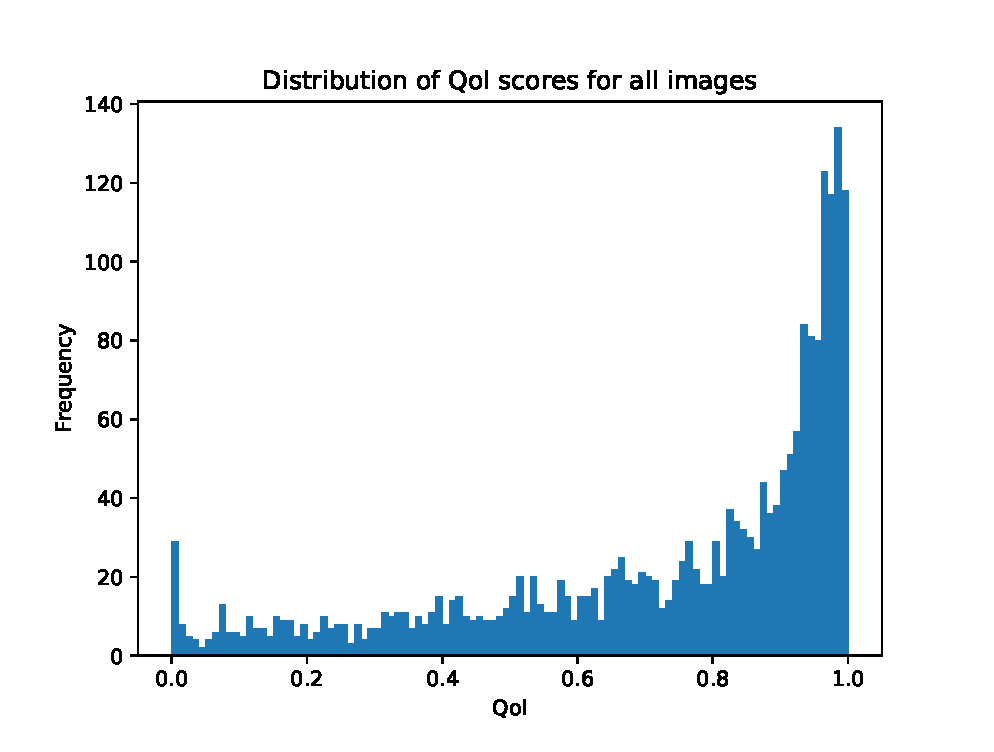
\includegraphics[scale=0.37]{img/SPIE/all_probs_smote_pca.eps}
  \caption{Distribution of scores on all the images}
  \label{fig:all_probs}
\end{subfigure}%
\begin{subfigure}{.5\textwidth}
  \centering
  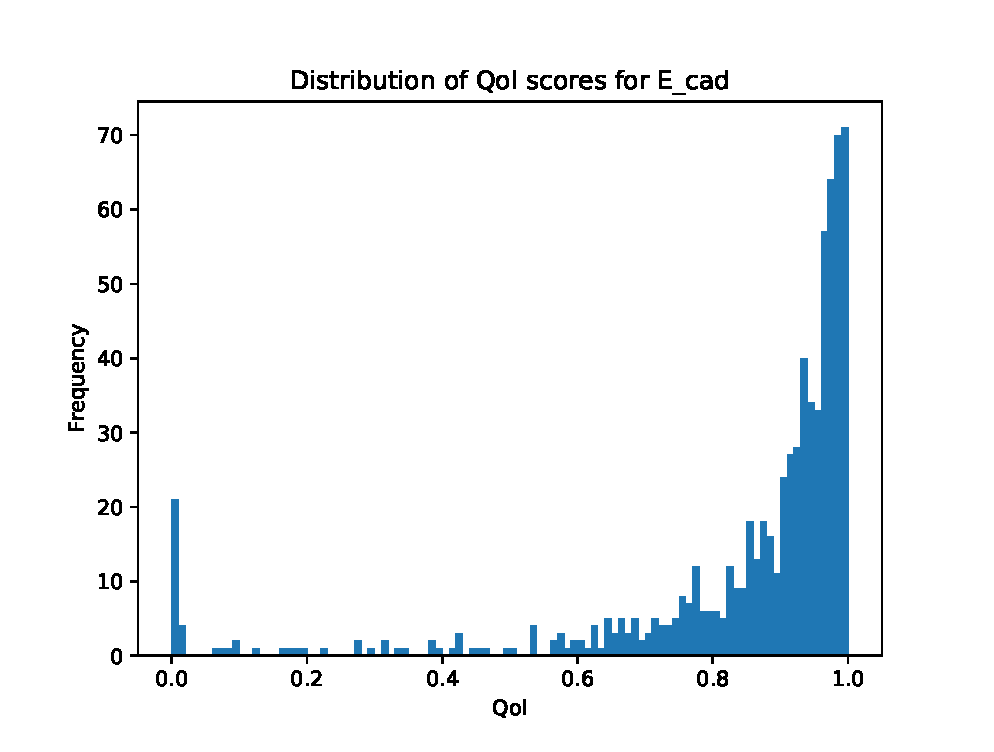
\includegraphics[scale=0.37]{img/SPIE/E_cad_probs_smote_pca.eps}
  \caption{Distribution of scores from E\_cad marker.}
  \label{fig:ecad_probs}
\end{subfigure}
\begin{subfigure}{.5\textwidth}
  \centering
  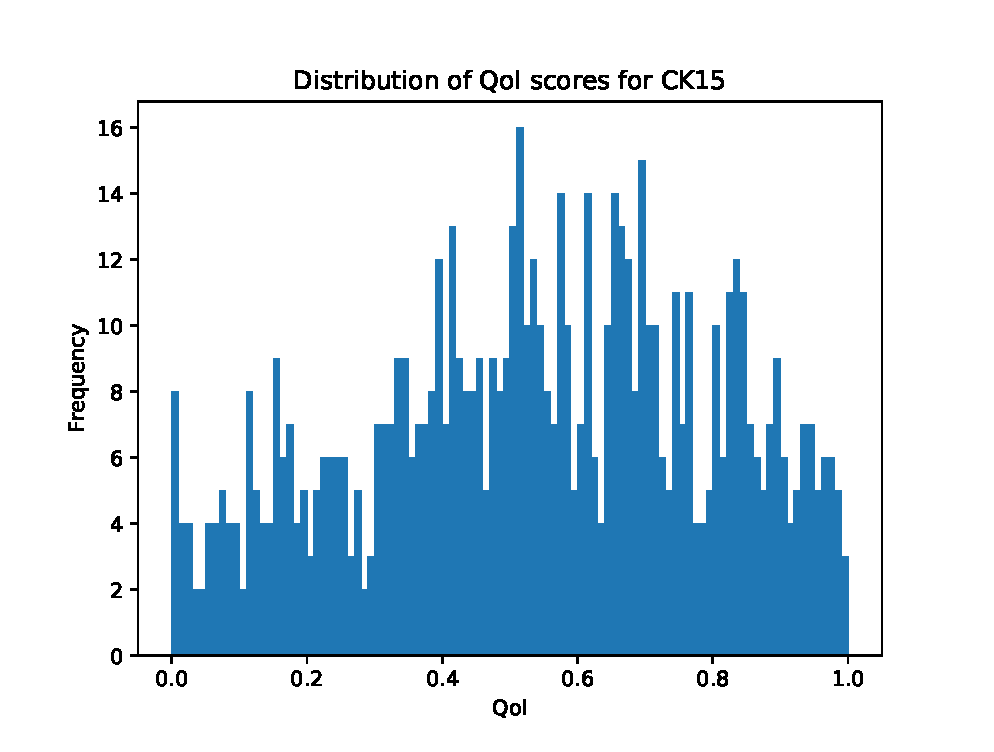
\includegraphics[scale=0.37]{img/SPIE/CK15_probs_smote_pca.eps}
  \caption{Distribution of scores from CK15 marker.}
  \label{fig:ck15_probs}
\end{subfigure}%
\begin{subfigure}{.5\textwidth}
  \centering
  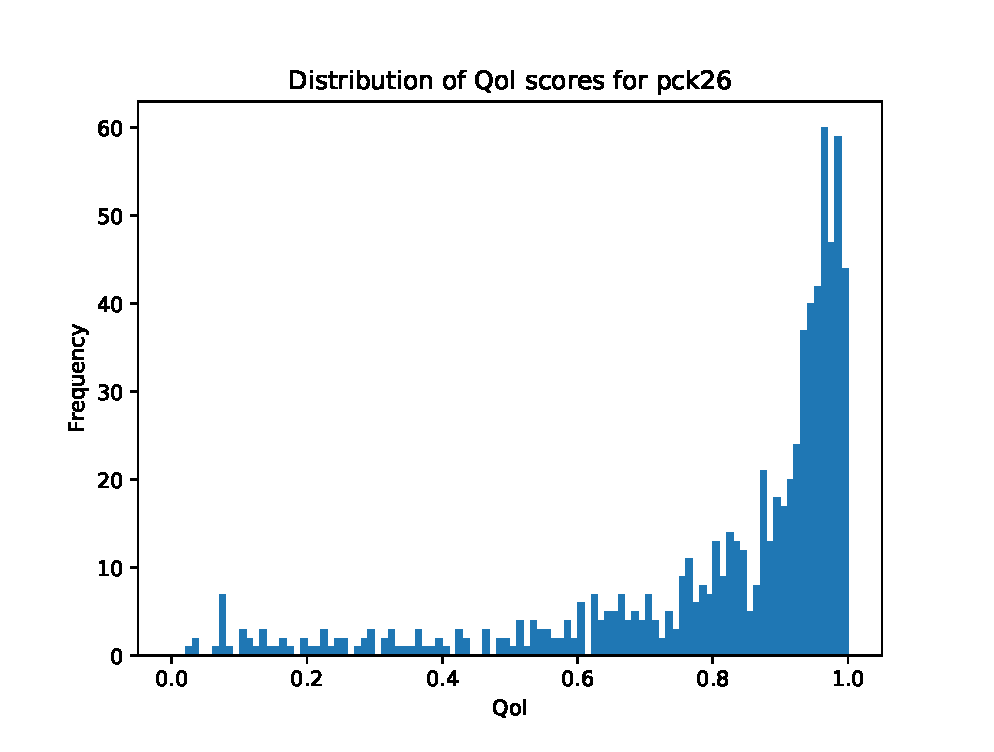
\includegraphics[scale=0.37]{img/SPIE/pck26_probs_smote_pca.eps}
  \caption{Distribution of scores from pck26 marker}
  \label{fig:pck26_probs}
\end{subfigure}
\caption{Distribution of \textit{QoI} scores on the images. According to the pathologist, the perceived quality of the images from the E\_cad and pck26 marker is good and the images from the CK15 marker has low signal and high noise in general.  This is reflected in the distribution of these markers}
\label{fig:distribution}
\end{figure}

The pathologist who labelled the images as \textit{good} or \textit{bad} based on the perceived quality of the images claimed that the images from the CK15 marker has more noise than images from E\_cad and pck26. This is exactly what we quantify using the \textit{QoI} score. The ratios of \textit{good} to \textit{bad} images for E\_cad, CK15 and pck26 are approximately 19:1, 19:1 and 17:1 respectively for the three markers. The difference in quality of the images are not captured by the distribution of the labels themselves. The distributions of the scores of the three markers in Fig. \ref{fig:distribution} clearly quantify this difference. We can see from Figs. \ref{fig:ecad_probs} and \ref{fig:pck26_probs} that the \textit{QoI} scores are skewed towards higher values close to one. On the other hand Fig. \ref{fig:ck15_probs} shows that there are a large number of images that maybe denoted as \textit{ugly}. The average values of the probabilities over all the images in a marker can be used to quantify the quality of the marker itself. In fact, the average values of the probabilities over all images in E\_cad, CK15 and pck26 are 0.85, 0.54 and 0.82 respectively.  Therefore, the quality of the markers E\_cad and pck26 is better than that of CK15. We divide the range of the scores into 3 equally spaced regions to demonstrate the difference between the three markers in more detail. The three regions are denoted as \textit{good} with a score range of 0.67 to 1, \textit{bad} with a range of 0 to 0.33 and \textit{ugly} with a range of 0.33 to 0.67. These values are chosen to demonstrate the differences between the markers. We discuss methods to select these thresholds later.

\begin{table}[ht!]
\centering
\caption{Percentage of the number of images that fall in the \textit{good}(0.67- 1), \textit{bad} (0 - 0.33) and \textit{ugly} (0.33 - 0.67)regions of the QoI score with respect to the 3 markers. The percentage values clearly quantify the claim that E\_cad is the least noisy followed by pck26 and CK15.}
\begin{tabular}{ |c|c|c|c|} 
 \hline
\textbf{Marker} & \textbf{good} (\%)& \textbf{bad} (\%) & \textbf{ugly} (\%)\\ 
 \hline
E\_cad & 43.14 & 16.33 & 10.54\\
 \hline
pck26 & 40.15 & 19.52 & 18.61\\
 \hline
CK15 & 16.71 & 64.14 & 70.85\\
 \hline
 \end{tabular}
\label{table:scores}
\end{table}


Let's focus on the region between the scores of 0.33 and 0.67, which we may denote as the \textit{ugly} region of the \textit{QoI} score in Table \ref{table:scores}. The percentage of images from E\_cad, pck26 and CK15 that fall in this region are 16.33 \%, 19.52 \% and 64.14 \% respectively. These values also show that there are more contentious images  with respect to the \textit{QoI} score in CK15 than in E\_cad and pck26.
We also show  the distribution of the scores over all the images in the three markers in Fig. \ref{fig:all_probs}. The plot shows that most of the images have high quality. This is because images from E\_cad and pck26 which have high amounts of signal (according to the pathologist) account for two-thirds of the total data.
It is clear from the results that the \textit{QoI} score maybe used to quantify the amount of usable signal in the image.  The \textit{QoI}  provides an indication as to whether a particular sample may or may not be used in the analysis. 

There could be a number of different ways to use the \textit{QoI} scores usefully for performing analysis. In Table \ref{table:scores}, we selected the thresholds arbitrarily by dividing the range of the scores into 3 equally spaced regions - \textit{good}, \textit{bad} and \textit{ugly}.  A threshold maybe set on the QoI by the analyst and only those images above the threshold can be used for further analysis. Alternatively, a data-driven approach maybe used to leverage the \textit{QoI} score for performing further analysis. For example, the next step of the process maybe to classify the images into different grades of cancer.
In this step the \textit{QoI} score can be obtained for the dataset in question. The classification maybe started with a sample of images that have \textit{QoI} above a certain threshold. Then images are added to the training in batches based on the \textit{QoI} scores in a sequential manner. This procedure maybe repeated until the accuracy on the held out test set plateaus or decreases. This threshold could be used as the cutoff \textit{QoI} score to threshold the images for analysis. This is a way to not only use the good images, but also include the information from \textit{ugly} images into the post-processing analyses.

\section{Conclusions}
We introduce in this chapter a machine learning based score to quantify the perceived quality of an image.  The score is defined as the confidence of a data point to be classified as \textit{good} with respect to a classification algorithm, namely logistic regression . Images that have high or low information content are easy to label as good or bad respectively. A labeling of the \textit{ugly} class becomes dependent on the observer. Therefore computing a score is a more natural way of extracting this third class of images. The score helps us retrieve images that may have been discarded by a simple binary classification; or that may have gone unnoticed by a human eye. This score maybe used by medical practitoners to not only quantify the quality of an image but also the quality of a protein marker as a whole, as we demonstrate in the experiments section. Thus, this score maybe used to filter a dataset by only using image samples and markers that have usable information in them. We propose a data-driven approach to select an appropriate threshold selecting scheme. This will not only help increase the overall quality of analysis, but also remove the burden on pathologists to manually filter and select \textit{good} images from the dataset.
In this work, we show how to quantify the noise or error from image classification pipelines using the probabilities from machine learning. In the next chapter, we move down the image classification pipeline and show how to quantify the contributions of errors from different components of the image classification pipeline. 